\documentclass[11pt,a4paper]{article}

% ---------- PACKAGES ----------
\usepackage[margin=2.5cm]{geometry}   % reasonable page margins
\usepackage{graphicx}                 % \includegraphics
\usepackage{float}                    % H = “exactly here” placement
\usepackage{booktabs}                 % nicer tables
\usepackage{array}                    % custom table column widths
\usepackage[hidelinks]{hyperref}      % clickable refs, no coloured boxes
\usepackage{caption}                  % better caption formatting

\setlength{\parskip}{6pt}             % small breathing space between paragraphs

% -----------------------------------------------------------
%          D O C U M E N T
% -----------------------------------------------------------
\begin{document}
	
	% ------------------------- Title Page ---------------------
	\title{\textbf{E-Commerce Webshop Prototype\\UX Design Portfolio Report}}
	\author{Enrico Ebert \and Kristian Popov \and Glison Doci \and Orik Mazreku}
	\date{\today}
	\maketitle
	\thispagestyle{empty}
	\newpage
	
	% -------------------------- Contents ----------------------
	\setcounter{tocdepth}{2}
	\tableofcontents
	\newpage
	
	% ==========================================================
	\section{Summary of Requirements}\label{sec:project-overview}
	Our e-commerce webshop delivers a \emph{simple, modern, and fully responsive} shopping experience. Essential features—product search, category filtering, and a shopping cart—are complemented by smart extras such as a light/dark
	-mode toggle.
	
	\subsection*{Target Users}
	\begin{itemize}
		\item \textbf{Regular Shoppers} browsing on laptops or smartphones.
		\item \textbf{Store Administrators} managing catalogue and user data.
	\end{itemize}
	
	\subsection*{Application Goals}
	\begin{itemize}
		\item Clean, intuitive UI and navigation.
		\item Fast product search and category filtering.
		\item Secure account creation and sign-in.
		\item Complete cart and checkout flow.
		\item Admin panel for catalogue and order management.
		\item Light/dark-mode toggle.
		\item Fully responsive.

	\end{itemize}
	
	% ==========================================================
\section{User Interface Design}\label{sec:user-interface-design}

% =======================================================
% 1) HOME SCREEN  ---------------------------------------
% =======================================================
\subsection{Home Screen}\label{subsec:home-screen}

	\begin{figure}[H]
	\centering
	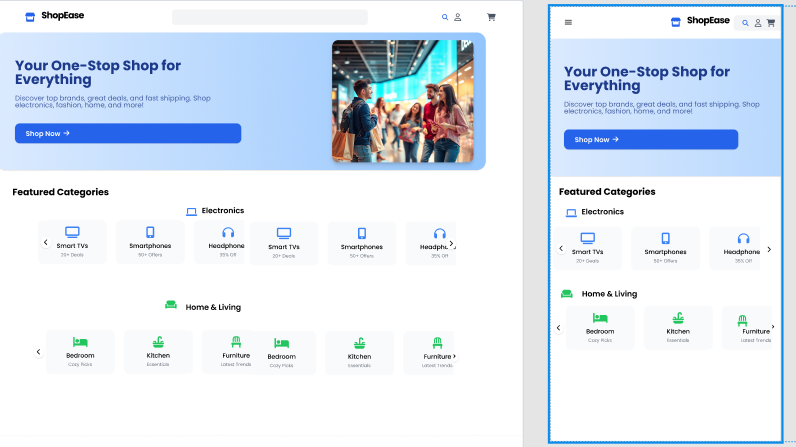
\includegraphics[width=\linewidth]{pictures/main/Home_figma}%
	\caption{Home screen in light mode .}
	\label{fig:ui-home}
\end{figure}

\paragraph{Explanation}%
The home page follows a classic information funnel: brand section~$\rightarrow$ value
proposition~$\rightarrow$ featured category. A single call-to-action
(*“Shop Now”*) avoids decision fatigue on first contact.  
All interactive controls (search, cart) are reachable within one
tap.

\begin{table}[H]
	\centering
	\caption{Home screen – elements and rationale}
	\label{tab:home-elements}
	\begin{tabular}{p{0.30\linewidth} p{0.60\linewidth}}
		\toprule
		\textbf{Design element} & \textbf{Purpose \& rationale} \\ \midrule
		Persistent top-bar      & Immediate access to search \& cart.\\
		Hero banner             & Communicates value proposition in one glance; accent colour draws the eye.\\
		Category carousel       & Promotes bestselling category; horizontal swipe invites mobile interaction.\\
		
		\bottomrule
	\end{tabular}
\end{table}
\subsection{Category Drawer (Hamburger / Desktop “Categories”)}

\begin{figure}[H]
	\centering
	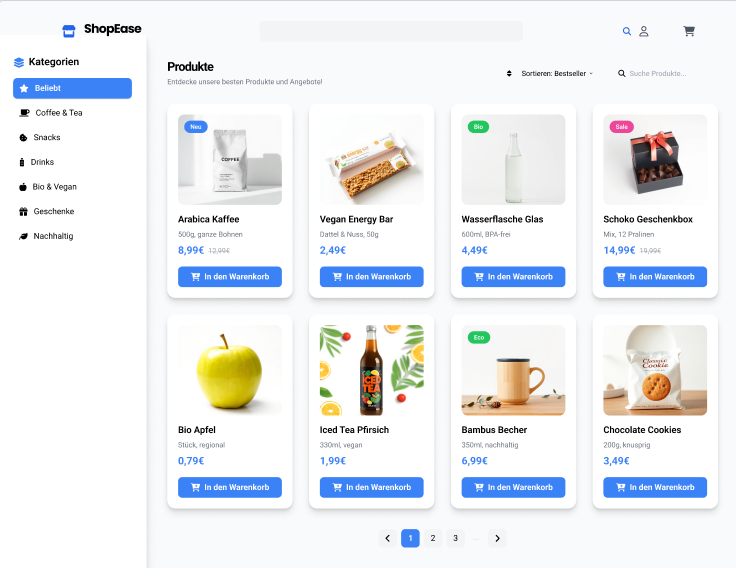
\includegraphics[width=\linewidth]{pictures/main/categories_Figma}%
	\caption{Off-canvas category drawer; mobile and desktop share the same component.}
	\label{fig:ui-category-drawer}
\end{figure}

\paragraph{Explanation}%
The drawer offers an identical filtering experience on both breakpoints:
a hamburger icon triggers it on mobile, while a “Categories” pill does so on
desktop. The underlying product grid is dimmed but remains in place, giving
immediate visual feedback when a category is selected.

\begin{table}[H]
	\centering
	\caption{Category drawer – elements and rationale}
	\label{tab:category-elements}
	\begin{tabular}{p{0.30\linewidth} p{0.60\linewidth}}
		\toprule
		\textbf{Design element} & \textbf{Purpose \& rationale} \\ \midrule

		Hamburger icon (mobile) & Saves horizontal space; familiar pattern. \\
		“Categories” pill (desktop) & reveals drawer on click. \\
		Accordion list          & Supports deep hierarchies without scrolling fatigue. \\
	
		\bottomrule
	\end{tabular}
\end{table}
% =======================================================
% 2) PRODUCT LIST SCREEN  -------------------------------
% =======================================================
\subsection{Product List Screen}

\begin{figure}[H]
	\centering
	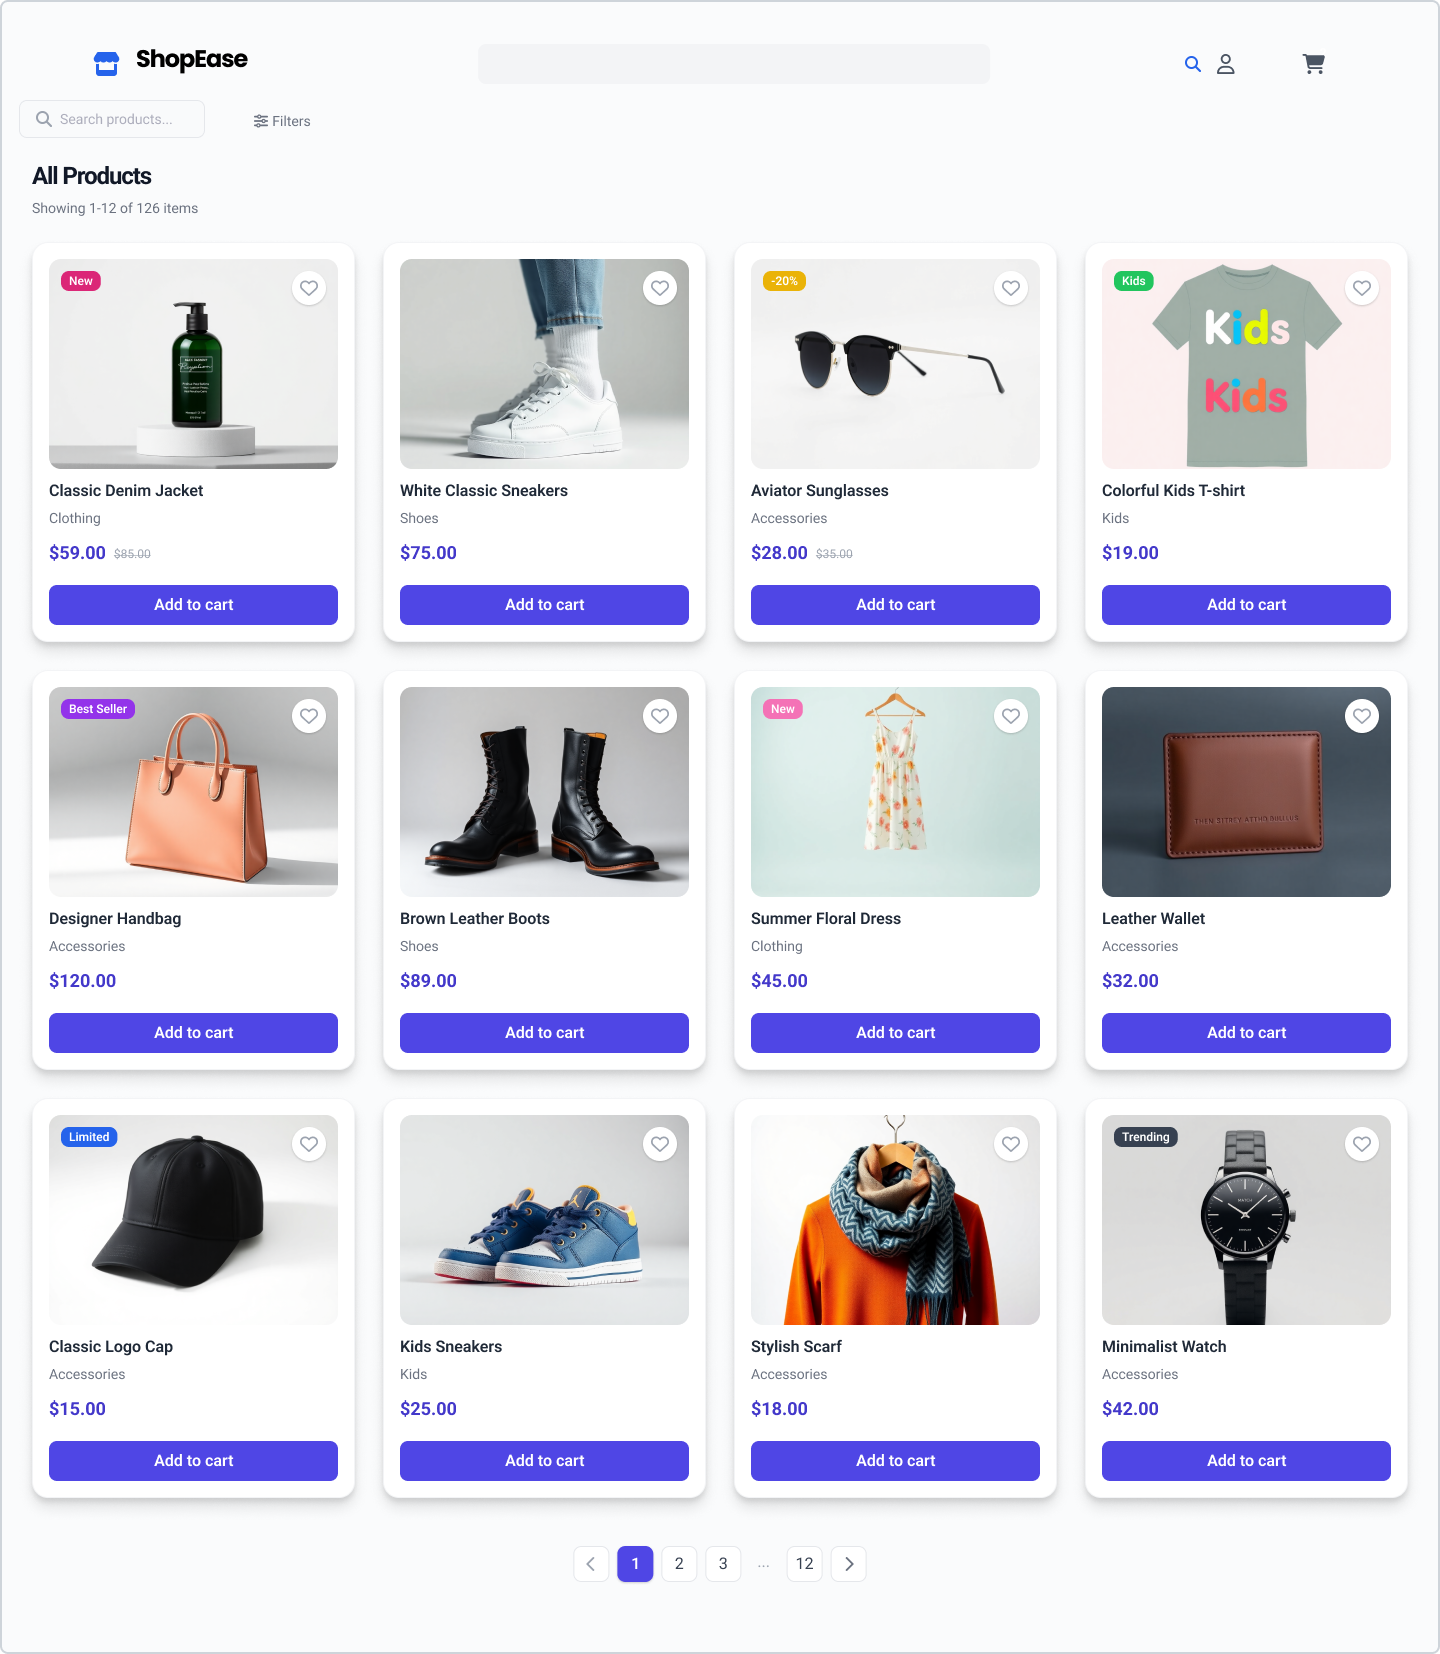
\includegraphics[width=\linewidth]{pictures/main/Product_List_Figma}%
	\caption{Product grid with search bar and category filter.}
	\label{fig:ui-products}
\end{figure}

\paragraph{Explanation}%
Users can search \emph{and/or} filter without leaving the page.  
The responsive grid keeps card proportions intact  focusable
cards maximise tap targets on touch devices.

\begin{table}[H]
	\centering
	\caption{Product list – elements and rationale}
	\label{tab:product-elements}
	\begin{tabular}{p{0.30\linewidth} p{0.60\linewidth}}
		\toprule
		\textbf{Design element} & \textbf{Purpose \& rationale} \\ \midrule
		Secondary navigation    & Lets users pivot between catalogue views .\\
		Search field            & Supports goal-oriented discovery; full-width on desktop, icon on mobile.\\
		Category dropdown       & Progressive narrowing while preserving context; default “Show all” reveals filter state.\\
	
	
		\bottomrule
	\end{tabular}
\end{table}

% =======================================================
% 2) SHOPPING CART SCREEN  -------------------------------
% =======================================================

	\subsection{Shopping Cart}\label{subsec:shopping-cart}

	\begin{figure}[H]
		\centering
		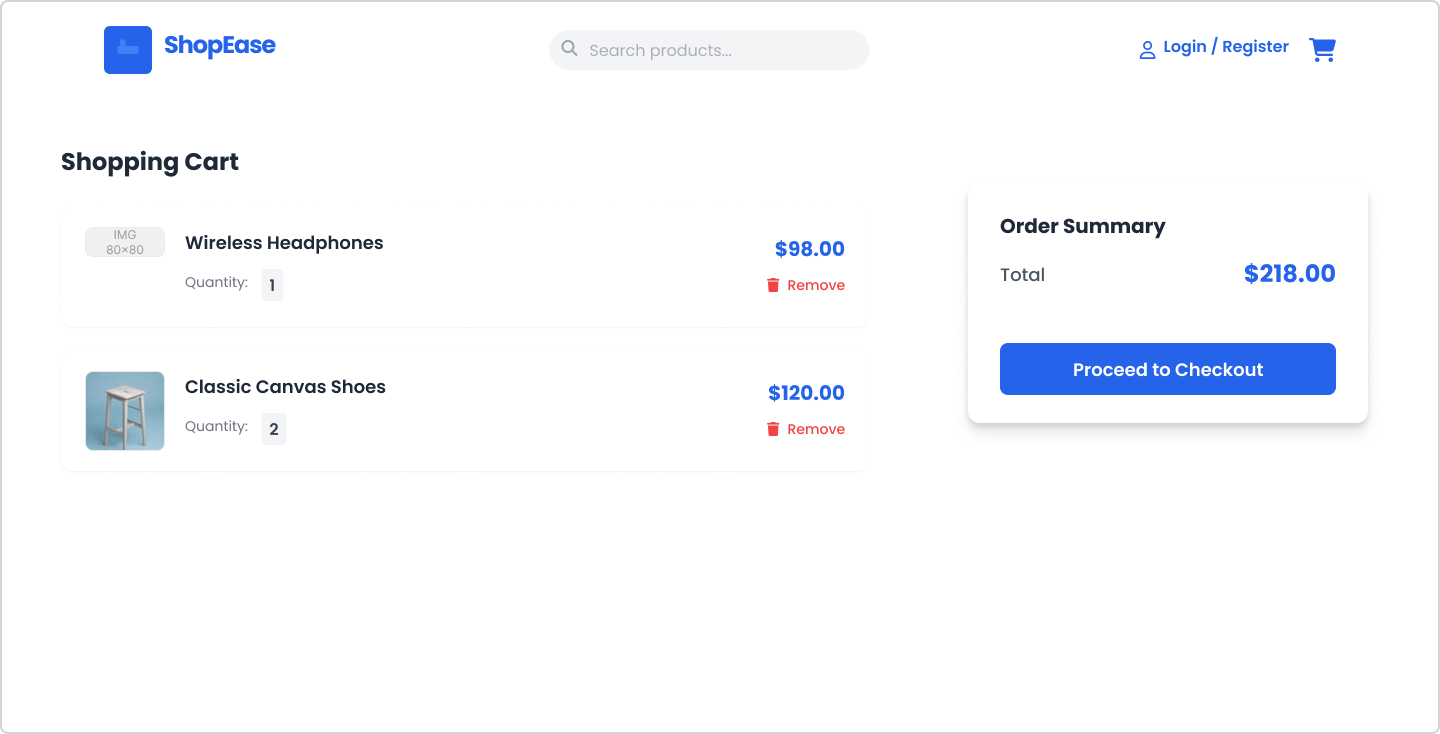
\includegraphics[width=\linewidth]{pictures/main/CartPage_Figma}%
		\caption{Shopping cart page with order summary and checkout.}
		\label{fig:ui-cart}
	\end{figure}

	\paragraph{Explanation}%
	The shopping cart page is designed for quick decision-making with a clear hierarchy:
	product list~$\rightarrow$ order summary~$\rightarrow$ checkout action. It minimizes distractions
	by focusing on removal options and a prominent *"Proceed to Checkout"* button.
	The layout ensures users can review costs and adjust items without leaving the page.

	\begin{table}[H]
		\centering
		\caption{Shopping cart – elements and rationale}
		\label{tab:cart-elements}

		\begin{tabular}{p{0.30\linewidth} p{0.60\linewidth}}
        	\toprule
        	\textbf{Design element} & \textbf{Purpose \& rationale} \\ \midrule
				Product rows            & Displays item names, images, and prices for verification. "Quantity" and "Remove" options allow instant edits. \\
        		Order summary           & Provides a clear breakdown of costs (e.g., subtotal, shipping) to reduce checkout abandonment. \\
        		Proceed to Checkout  & High-contrast button positioned last in the visual flow to guide users toward conversion. \\
        		Login/Register prompt   & Encourages account creation after cart engagement to avoid early friction. \\
        	\bottomrule
    	\end{tabular}

	\end{table}


% =======================================================
% 2) REGISTER/LOGIN SCREEN  -------------------------------
% =======================================================

	\subsection{Login \& Registration}\label{subsec:login-register}

	\begin{figure}[H]
		\centering
		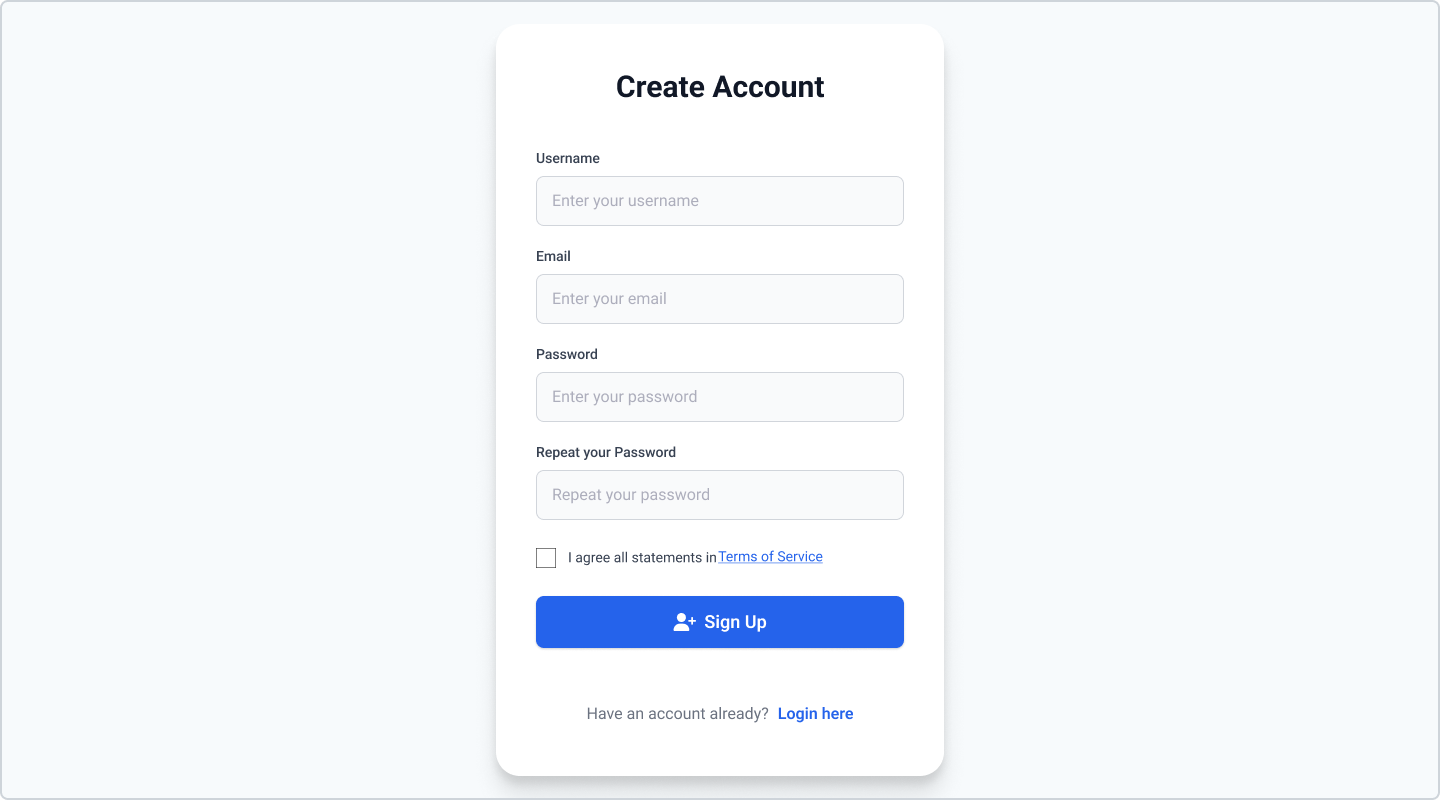
\includegraphics[width=1.0\linewidth]{pictures/main/RegisterAccount_Figma}%
		\caption{Login screen with email/password fields and registration prompt.}
		\label{fig:ui-login}
	\end{figure}

	\paragraph{Explanation}%
	The login page prioritizes simplicity with a minimal form (email/password).
	Register guides new users to account creation. 
	\begin{table}[H]
		\centering
		\caption{Login screen – elements and rationale}
		\label{tab:login-elements}
		\begin{tabular}{p{0.30\linewidth} p{0.60\linewidth}}
			\toprule
			\textbf{Design element} & \textbf{Purpose \& rationale} \\ \midrule
			Email/Password fields   & Standardized input format for familiarity and quick completion. \\
			Login button       & Primary action styled for prominence; triggers authentication. \\
			Register prompt        & Registration of new users. \\
			Minimal layout         & Focuses attention on form completion. \\
			\bottomrule
		\end{tabular}
	\end{table}
	
	
	\section{Admin Design}\label{sec:admin-design}
	\vspace{0.3cm}
	
	
	\subsection{Admin Architecture}\label{subsec:admin-architecture}
	The admin dashboard provides a comprehensive overview of key business metrics. It features six distinct pages, accessible via the left-hand navigation bar:
	\begin{itemize}
		\item \textbf{Overview} - This is the primary landing page, offering a high-level summary of performance.
		\item \textbf{Products} - This page would likely allow administrators to view, add, edit, or delete products.
		\item \textbf{Customers} - This page would provide tools for managing customer
		\item \textbf{Account} - This page contains settings related to the administrator's account, including profile information, profile settings, password management, notification preferences, social account management, and the option to delete the account.
		\item \textbf{Settings} - This page contains global settings for the platform, such as language and timezone preferences, date and time formats, accessibility options, and other general configurations.
	\end{itemize}
	\subsection{Overview Page}\label{subsec:overview-page}
	
	
	\begin{figure}[h]
		\centering
		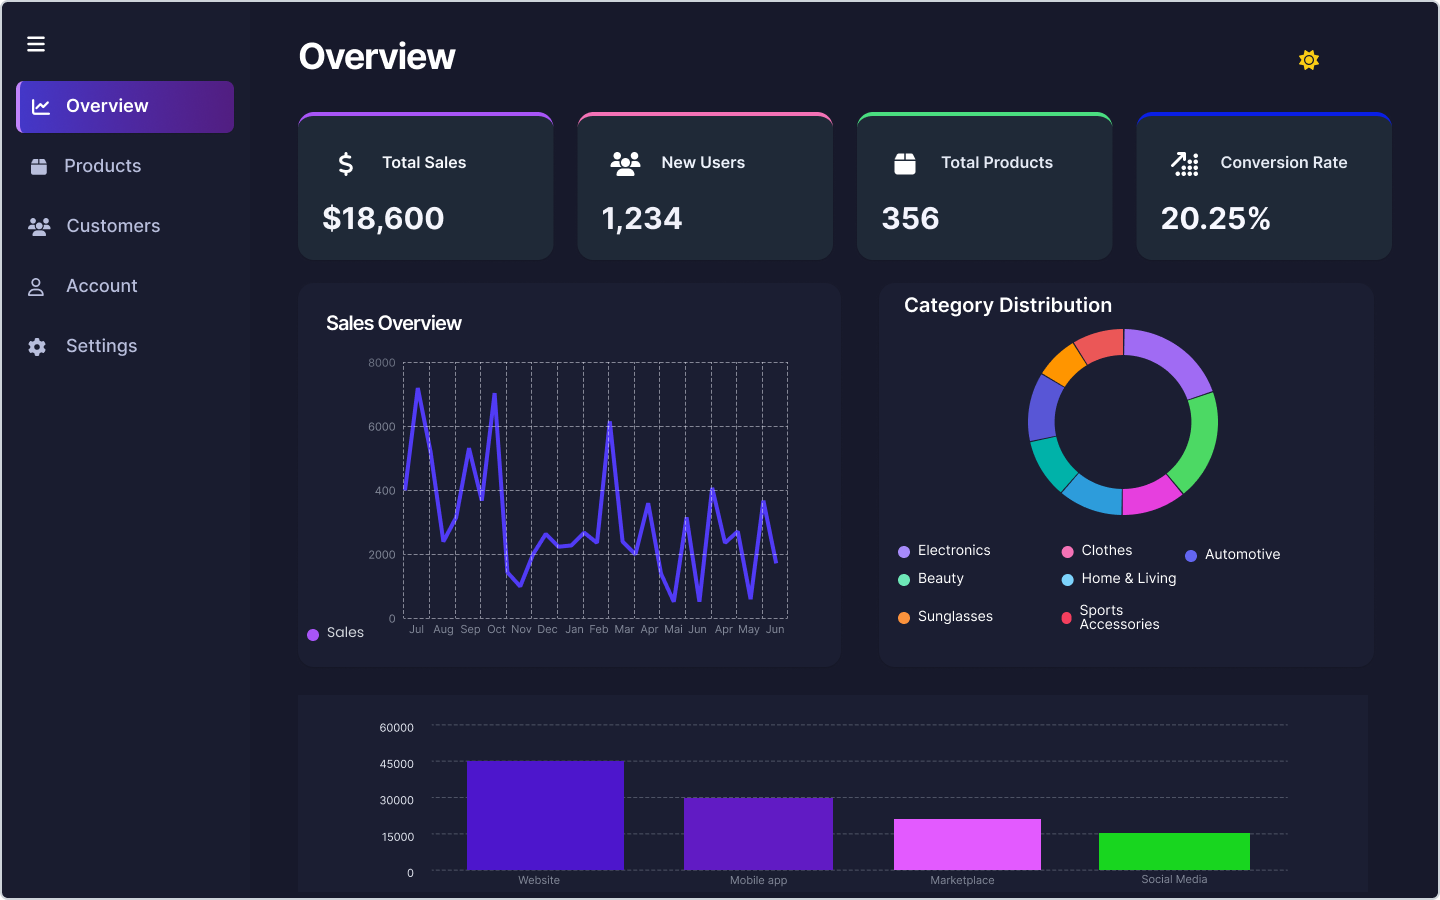
\includegraphics[width=1\textwidth]{pictures/admin/Overview_Admin}
		\caption{Overview page in dark mode}\label{fig:figure1}
	\end{figure}
	\vspace{0.3cm}
	The Overview Page serves as an analytics dashboard where administrators can track the platform’s performance in real time. \\ \\
	At the top, four distinct cards display key performance indicators (KPIs):
	\begin{itemize}
		\item \textbf{Total Sales} – Displays the total revenue generated during the current month.
		\item \textbf{New Users} – Shows the number of new user accounts created this month.
		\item \textbf{Total Products} – Indicates the total number of products available in the webshop.
		\item \textbf{Conversion Rate} – Represents the percentage of users who completed a purchase out of the total visitors.
	\end{itemize}
	Below the KPI cards, three graphical components offer deeper insights:
	\begin{itemize}
		\item \textbf{Sales Overview (Line Graph)} - Visualizes monthly revenue trends across different months.
		\item \textbf{Category Distribution (Pie Chart)} - Shows the proportion of sales by product category, highlighting which categories perform best.
		\item \textbf{Sales by Channel (Bar Chart)} - Breaks down sales by purchase channel—Website, Mobile App, Marketplace, and Social Media—revealing which channels drive the most revenue.
	\end{itemize}
	
	
	\subsection{Product Page}\label{subsec:product-page}
	\begin{figure}[h]
		\centering
		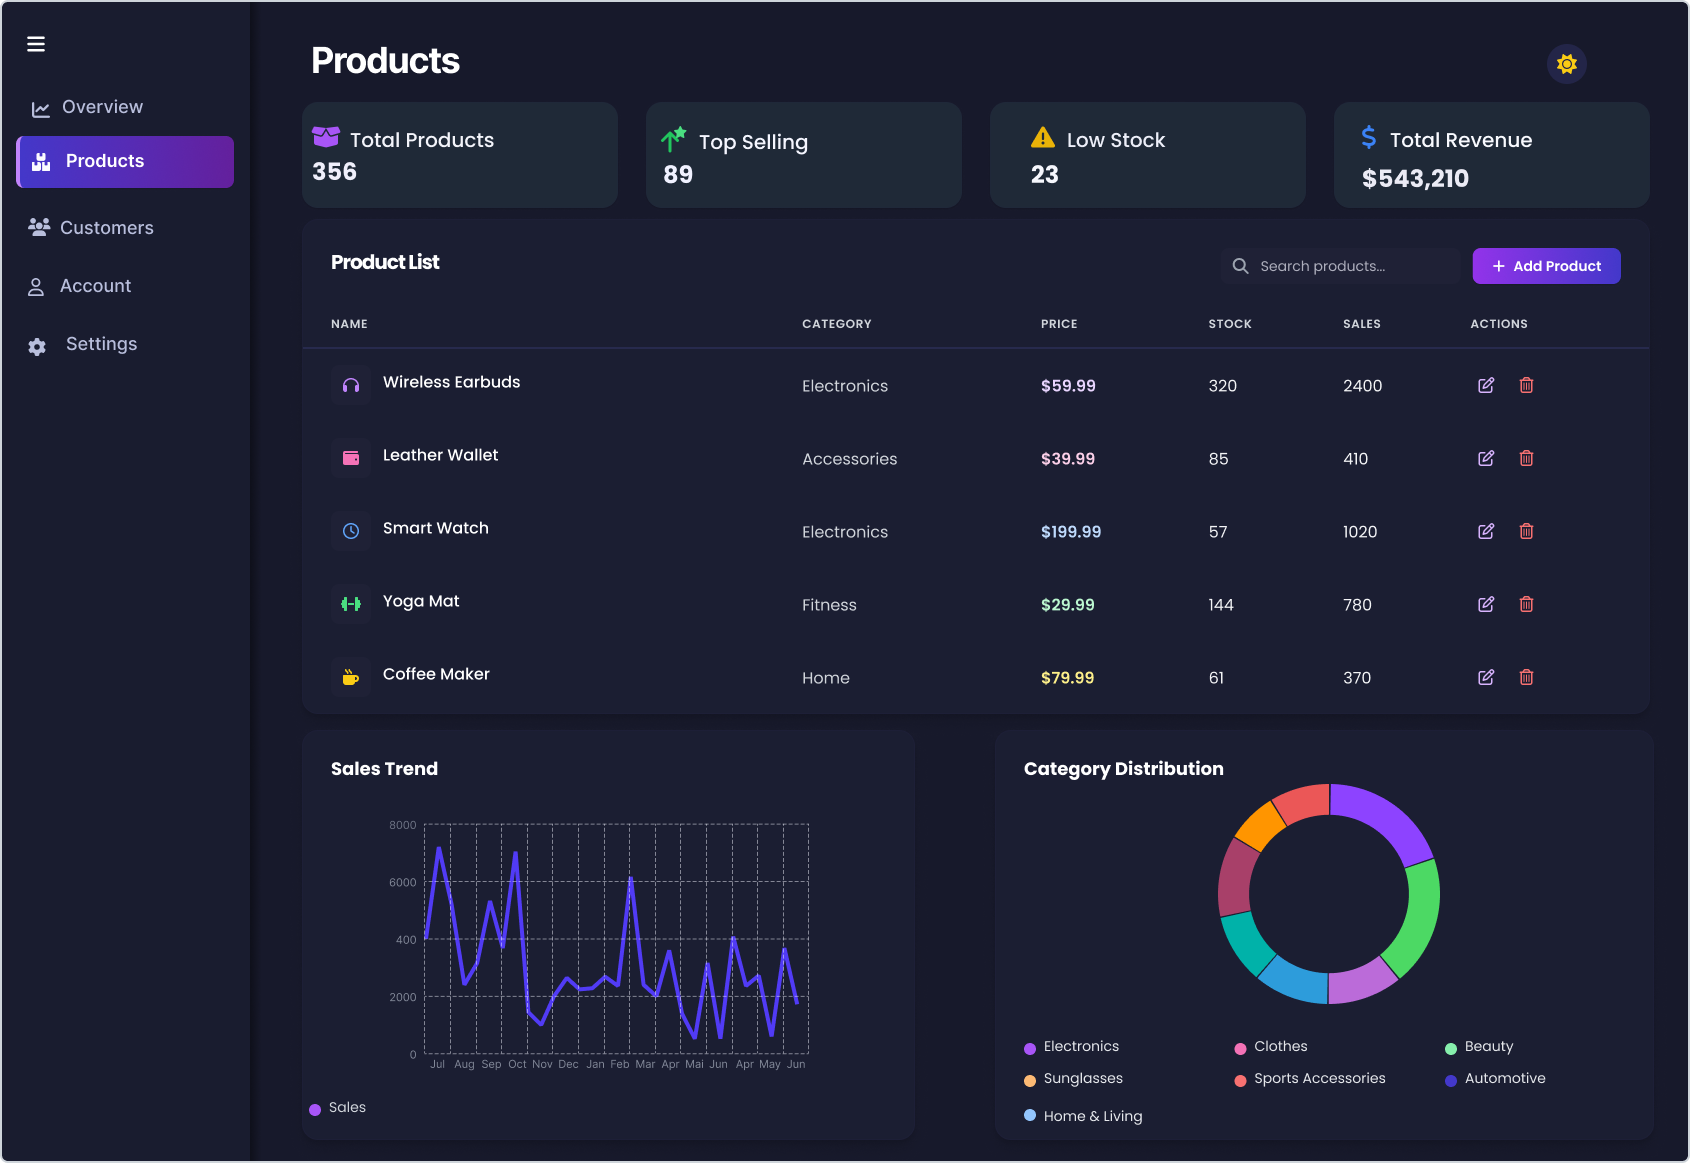
\includegraphics[width=0.9\textwidth]{pictures/admin/Products_Admin}
		\caption{Products page}\label{fig:figure2}
	\end{figure}
	This page allows the administrator to manage products efficiently while monitoring key performance metrics. \\ \\
	\textbf{KPI Cards} \\
	At the top, four distinct cards display key performance indicators:
	\begin{itemize}
		\item \textbf{Total Products} – Shows the total number of products currently in the webshop.
		\item \textbf{Top Selling} – Highlights the product with the highest number of sales.
		\item \textbf{Low Stock} – Indicates the number of products with low inventory.
		\item \textbf{Total Revenue} – Displays the total revenue generated for the current day.
	\end{itemize}
	Product List Section
	Beneath the KPI cards is a prominent Product List presented in a tabular format. This section provides a detailed overview of all products.
	\begin{itemize}
		\item \textbf{Search Bar} – Located on the right, it allows real-time filtering of the products as the admin types.
		\item \textbf{Add Product Button} – Positioned next to the search bar, this rectangular button enables the admin to add a new product. Upon clicking, a form/modal appears for entering the product’s details.
	\end{itemize}
	The table contains the following headers:
	\begin{itemize}
		\item \textbf{NAME} – Product name.
		\item \textbf{CATEGORY} – The category the product belongs to.
		\item \textbf{PRICE} – Product price.
		\item \textbf{STOCK} – Current inventory count.
		\item \textbf{SALES} – Number of units sold.
		\item \textbf{ACTIONS} – Contains two buttons:
		\begin{itemize}
			\item \textbf{Edit} – Opens a form to modify product details.
			\item \textbf{Delete} – Removes the product from the list.
		\end{itemize}
	\end{itemize}
	At the bottom of the page, two main charts provide insights into product performance:
	\begin{itemize}
		\item \textbf{Sales Trend (Line Graph)} - Displays sales progression over time, helping track revenue trends.
		\item \textbf{Category Distribution (Pie Chart)} - Visualizes how sales are distributed across product categories.
	\end{itemize}
	
	
	\subsection{Customers Page}\label{subsec:customers-page}
	\begin{figure}[h]
		\centering
		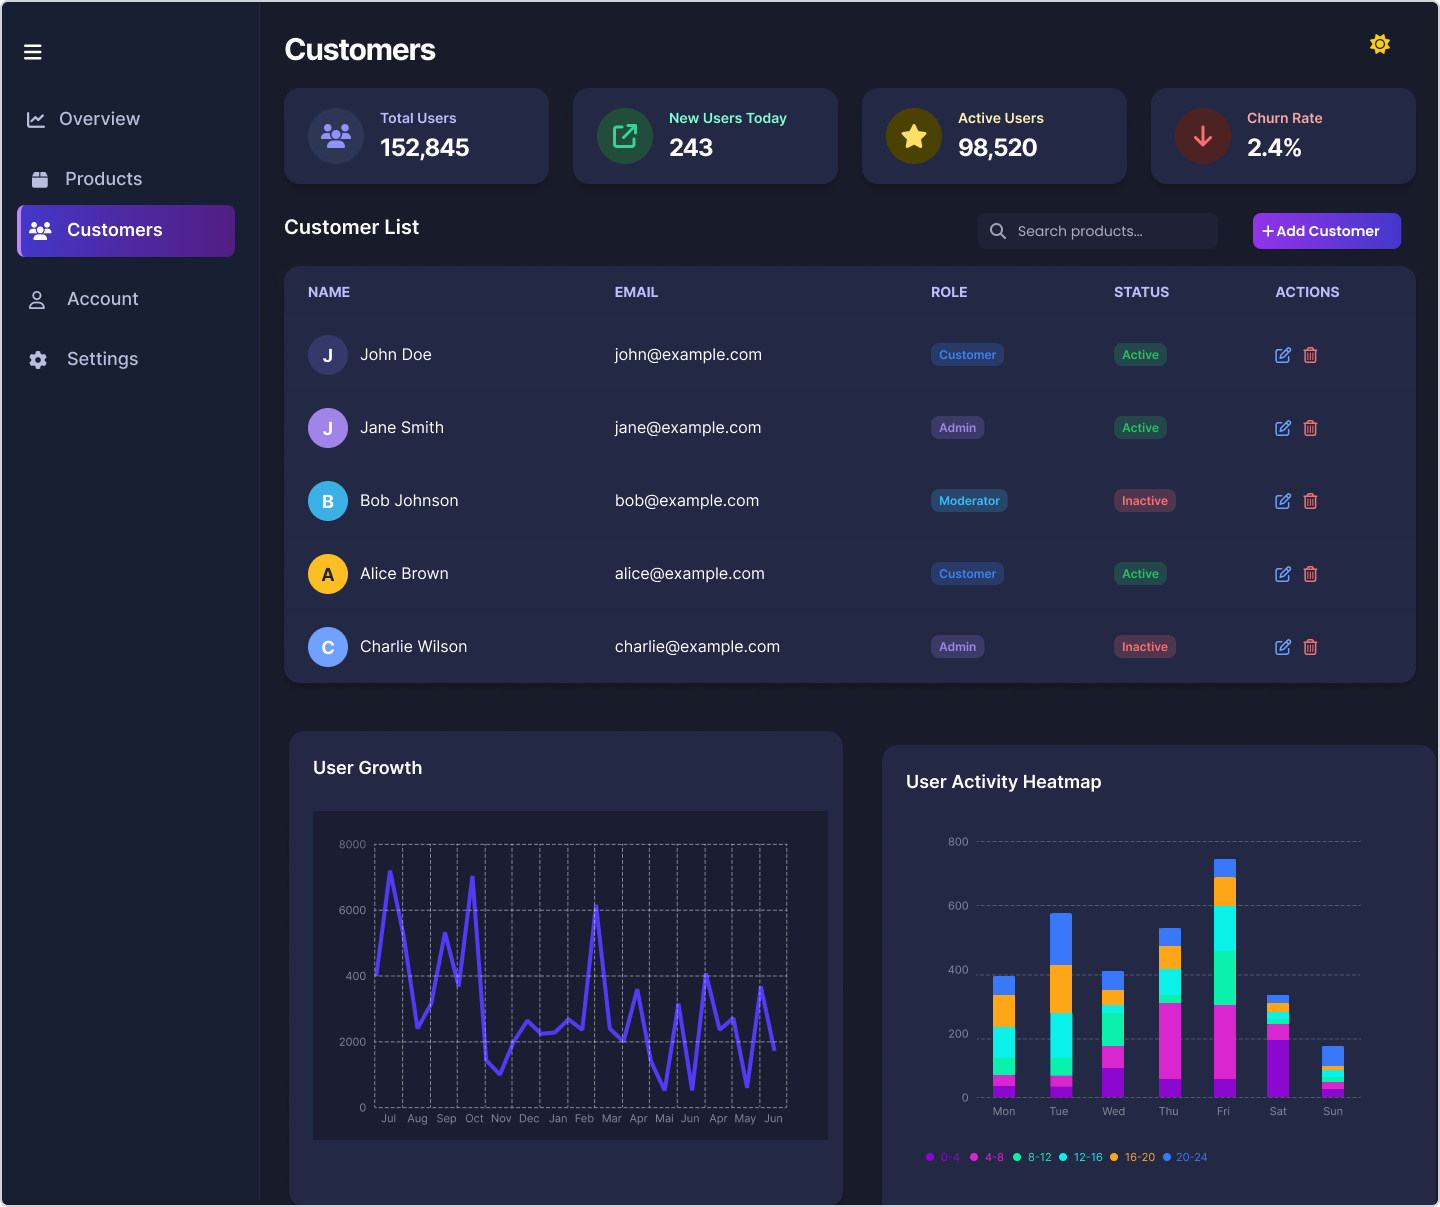
\includegraphics[width=0.9\textwidth]{pictures/admin/Customers_Admin}
		\caption{Customers page}\label{fig:figure3}
	\end{figure}
	This page allows the administrator to manage customers/users efficiently. \\ \\
	At the top, four distinct cards display key performance indicators:
	\begin{itemize}
		\item \textbf{Total Users} - Shows the total number of registered customers/users.
		\item \textbf{New Users Today} - Displays the number of users who registered today.
		\item \textbf{Active Users} - Indicates the current number of active users.
		\item \textbf{Churn Rate} - Shows the percentage of users who have stopped engaging with the platform.
	\end{itemize}
	Customer List Section
	Beneath the KPI cards is a prominent Customer List presented in a tabular format, providing a detailed overview of all registered users.
	\begin{itemize}
		\item \textbf{Search Bar} – Located on the right, it allows real-time filtering of the products as the admin types.
		\item \textbf{Add Customer Button} – Positioned next to the search bar, this rectangular button enables the admin to add a new customer/user. Upon clicking, a form/modal appears for entering the product’s details.
	\end{itemize}
	The table includes the following columns:
	\begin{itemize}
		\item \textbf{NAME} – Full name of the customer.
		\item \textbf{EMAIL} – Email address of the customer.
		\item \textbf{ROLE} – Assigned role (e.g., User, Admin).
		\item \textbf{STATUS} – Account status (e.g., Active, Inactive).
		\item \textbf{ACTIONS} – Contains two buttons:
		\begin{itemize}
			\item \textbf{Edit} – Opens a form to modify customer details.
			\item \textbf{Delete} – Removes the customer from the list.
		\end{itemize}
	\end{itemize}
	At the bottom of the page, two visualizations provide additional insights:
	\begin{itemize}
		\item \textbf{User Growth (Line Graph)} - Displays the growth in user registrations over time.
		\item \textbf{User Activity Heatmap (Bar Chart)} - Shows the distribution of user activity across different age groups or time periods.
	\end{itemize}
	
	
	\subsection{Account Page}\label{subsec:account-page}
	
	\subsubsection{Profile}
	
	\vspace{0.5cm}
	\begin{figure}[h]
		\centering
		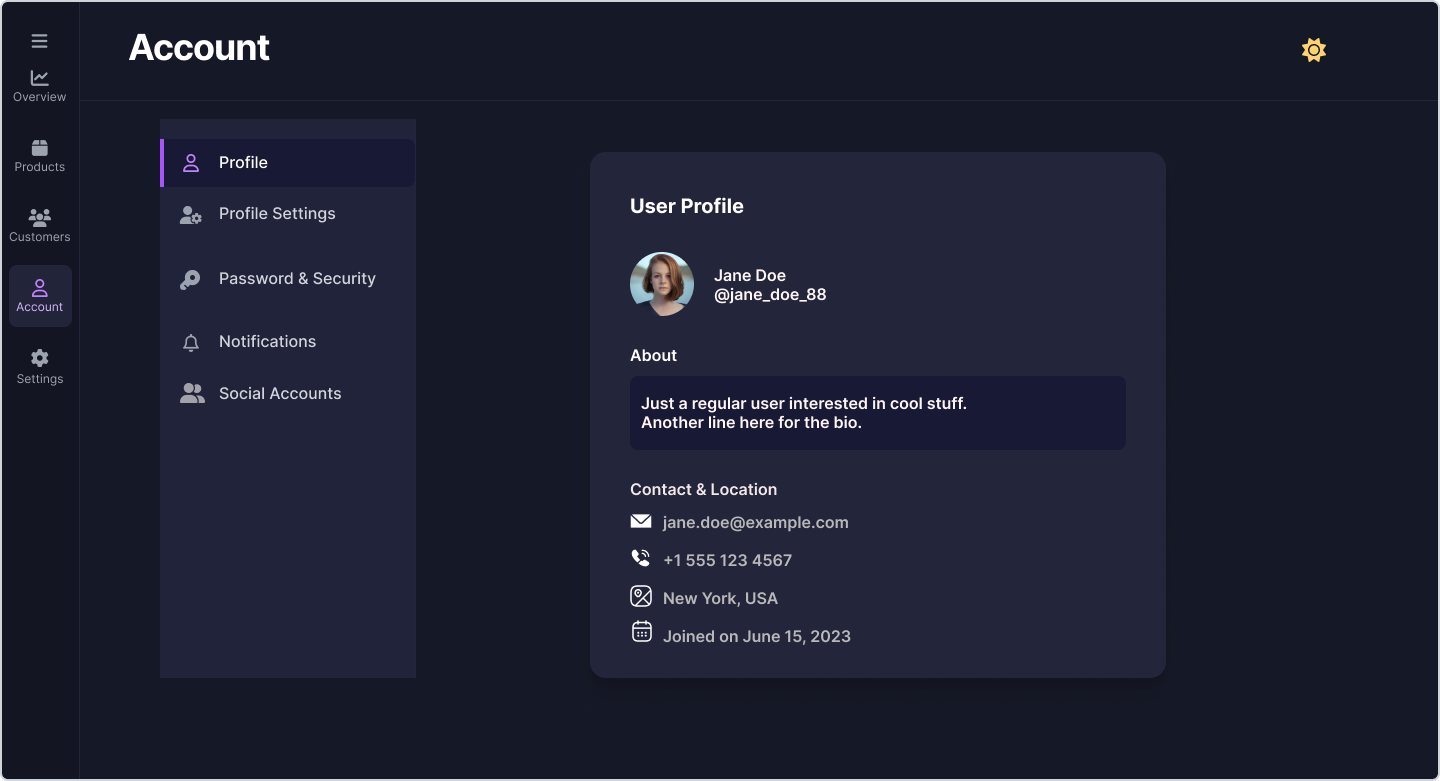
\includegraphics[width=0.8\textwidth]{pictures/admin/Profile_Admin}
		\caption{Profile page}\label{fig:figure4}
	\end{figure}
	This page displays the admin’s personal information, including name, email address, phone number, country, and the date the account was created.
	
	\subsubsection{Profile Settings}
	\begin{figure}[h]
		\centering
		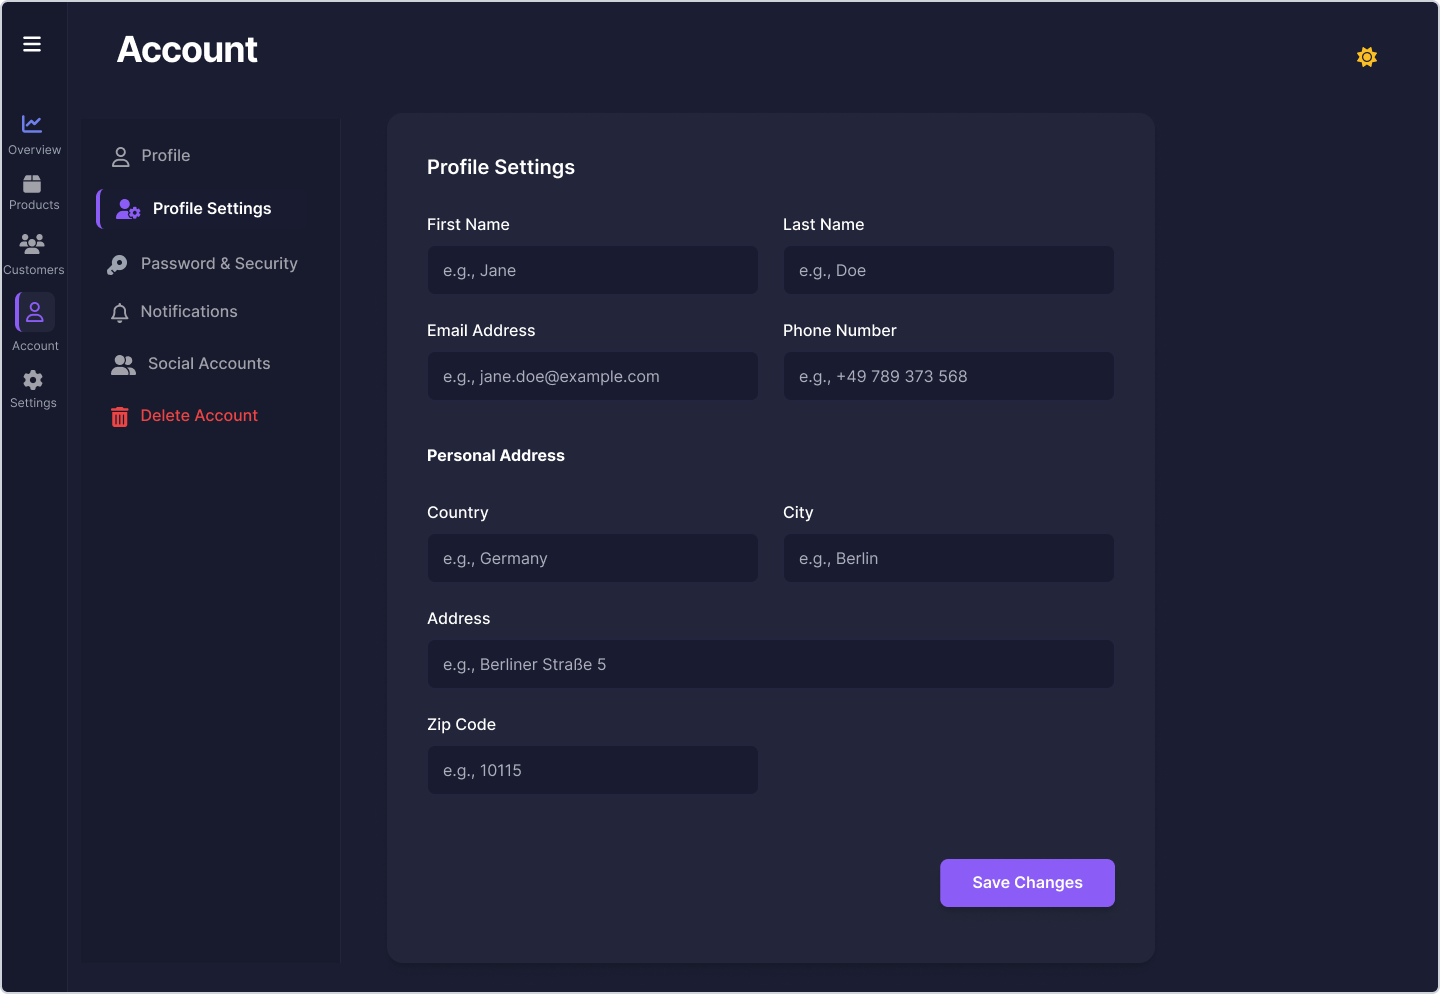
\includegraphics[width=0.8\textwidth]{pictures/admin/ProfileSettings_Admin}
		\caption{Profile settings page}\label{fig:figure5}
	\end{figure}
	This page allows the administrator to view and update their personal information.
	It is organized into two main sections: \\
	\textbf{Personal Information} \\
	The admin can update the following fields: Name, Email Address, Phone Number \\ \\
	\textbf{Address Information} \\
	This section enables the admin to manage their address details:Country, City, Street Address, ZIP Code \\ \\
	A \textbf{"Save Changes"} button is available at the bottom of the page to apply updates.
	\subsubsection{Password \& Security}
	\begin{figure}[h]
		\centering
		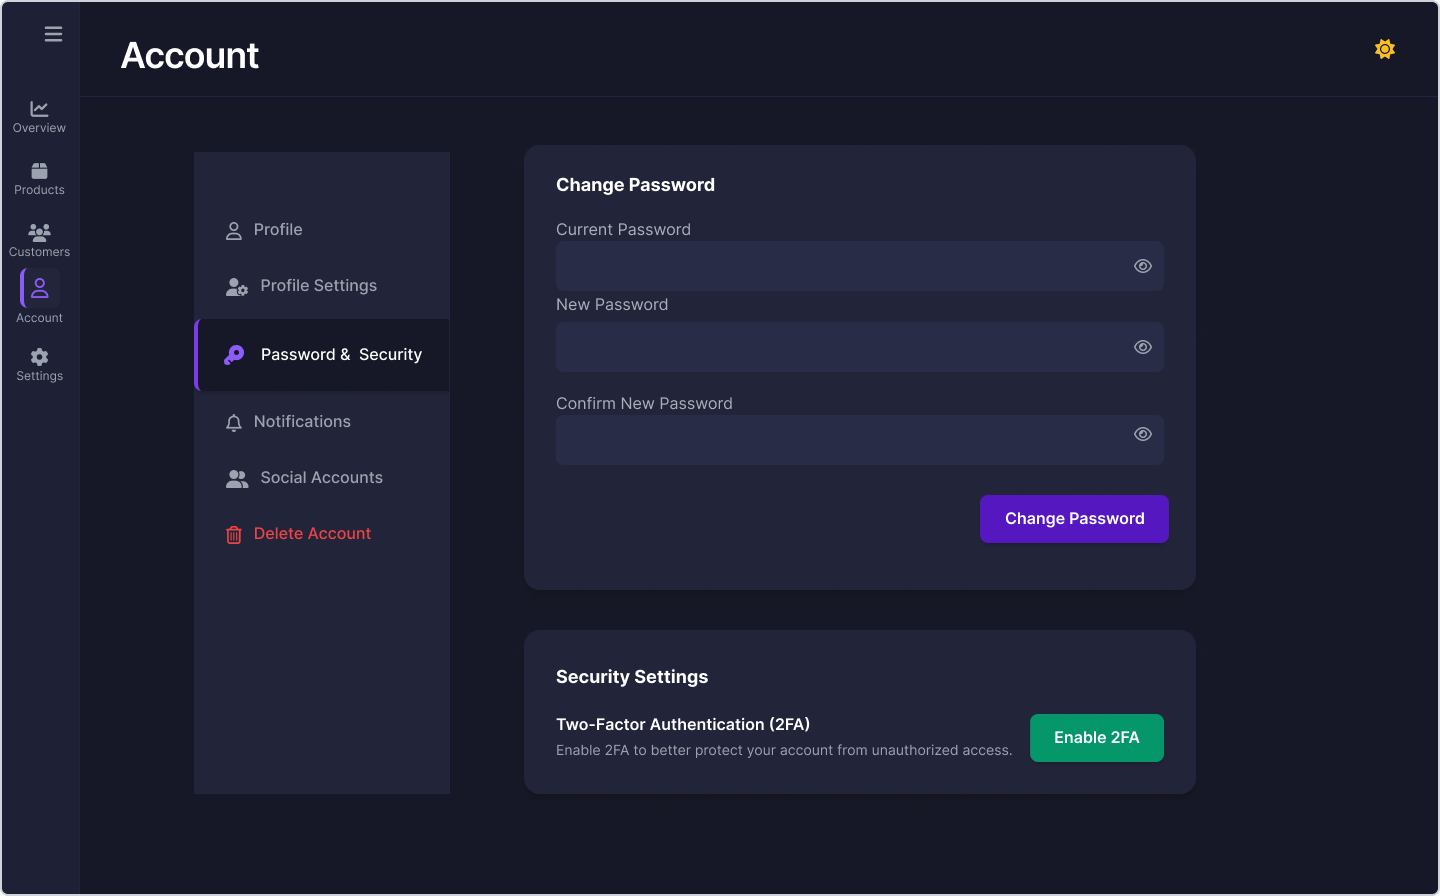
\includegraphics[width=0.8\textwidth]{pictures/admin/Password_Admin}
		\caption{Password and Security page}\label{fig:figure6}
	\end{figure}
	This page allows the administrator to change their password and manage two-factor authentication (2FA). It is organized into two main sections: \\ \\
	\textbf{Change Password} \\
	The admin can update their login password by entering:
	\begin{itemize}
		\item The current password
		\item The new password
		\item Confirm new password
	\end{itemize}
	A \textbf{"Change Password"} button is provided at the bottom of this section to apply the update. \\ \\
	\textbf{Two-Factor Authentication (2FA)} \\
	This section enables the administrator to enhance account security with 2FA. It includes: A toggle or switch to enable or disable 2FA
	
	
	\subsubsection{Notifications}
	\begin{figure}[h]
		\centering
		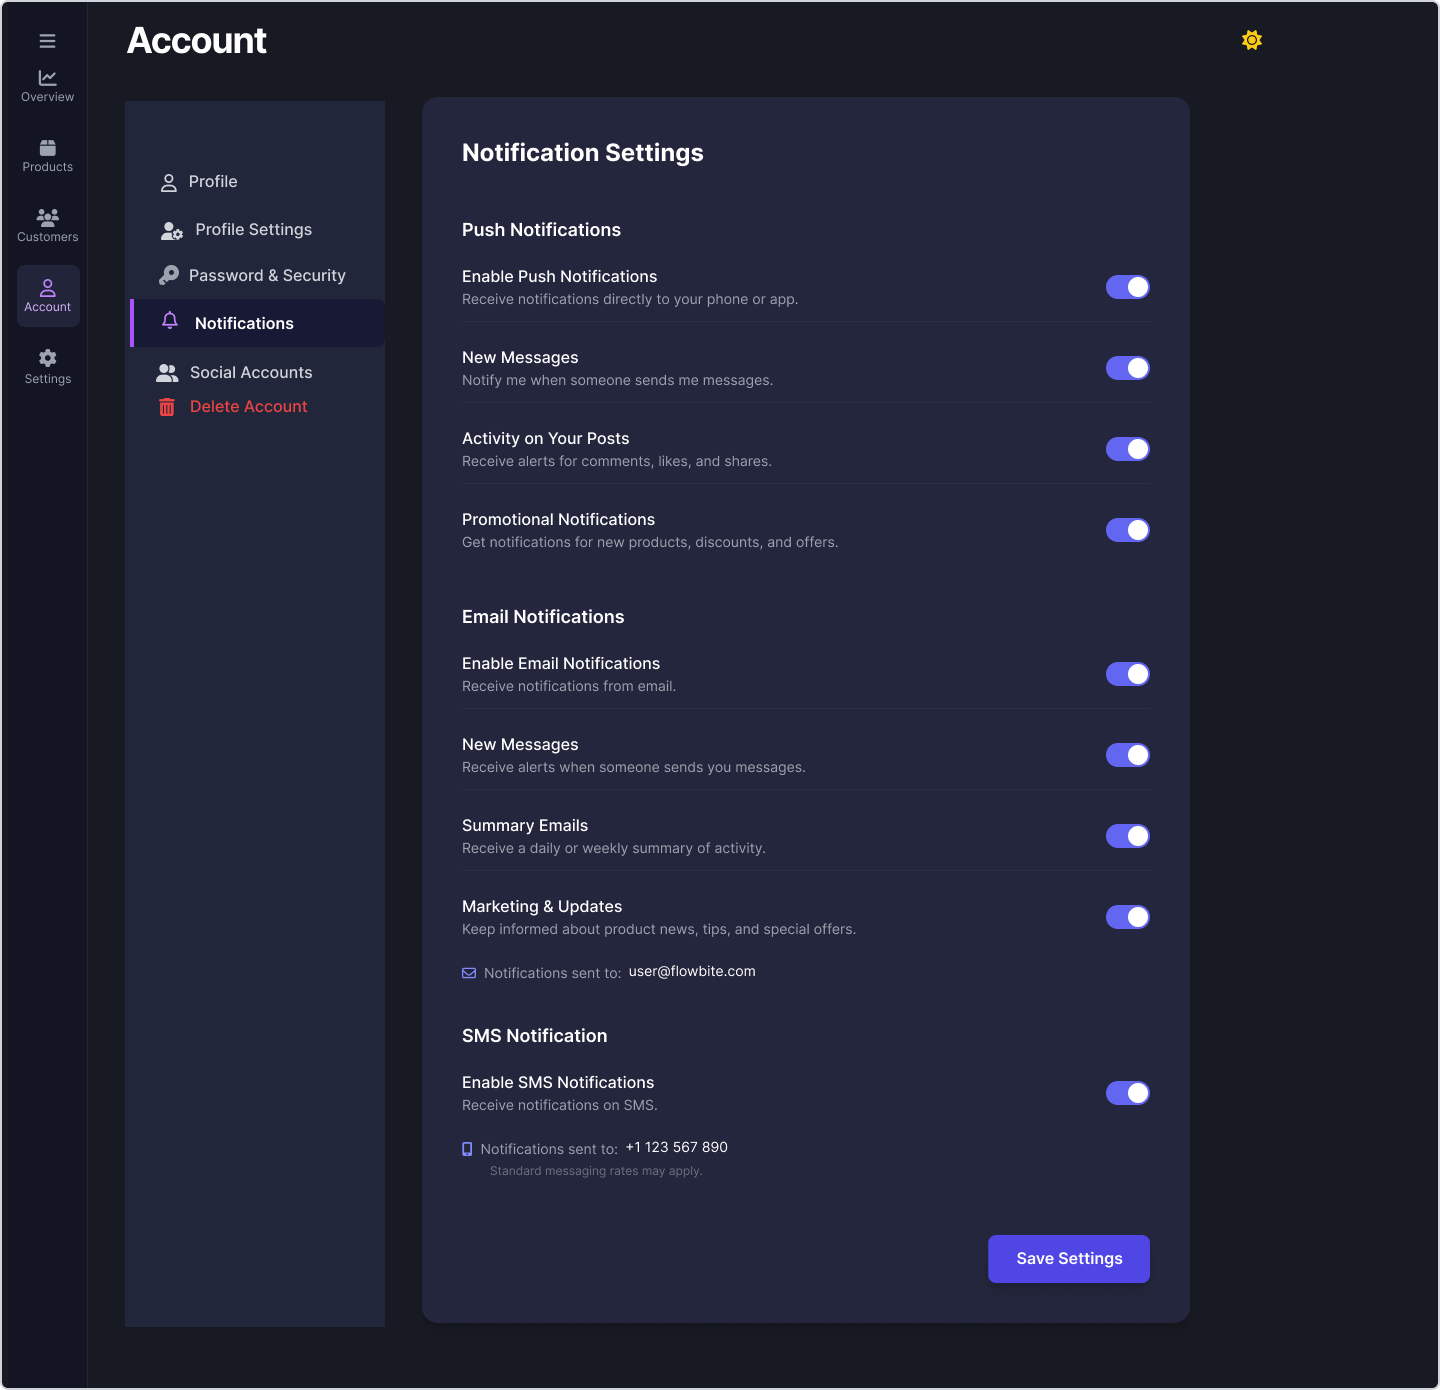
\includegraphics[width=0.8\textwidth]{pictures/admin/Notifications_Admin}
		\caption{Notifications page}\label{fig:figure7}
	\end{figure}
	This page displays notification settings.
	It includes sections for Push Notifications, Email Notifications, and SMS Notifications. Each section has toggles to enable or disable different types of notifications, such as new messages, activity on posts, promotional updates, summary emails, and marketing updates. It also shows the email address and phone number where notifications are sent, and a "Save Settings" button at the bottom to apply the changes.
	\subsubsection{Social Accounts}
	\begin{figure}[h]
		\centering
		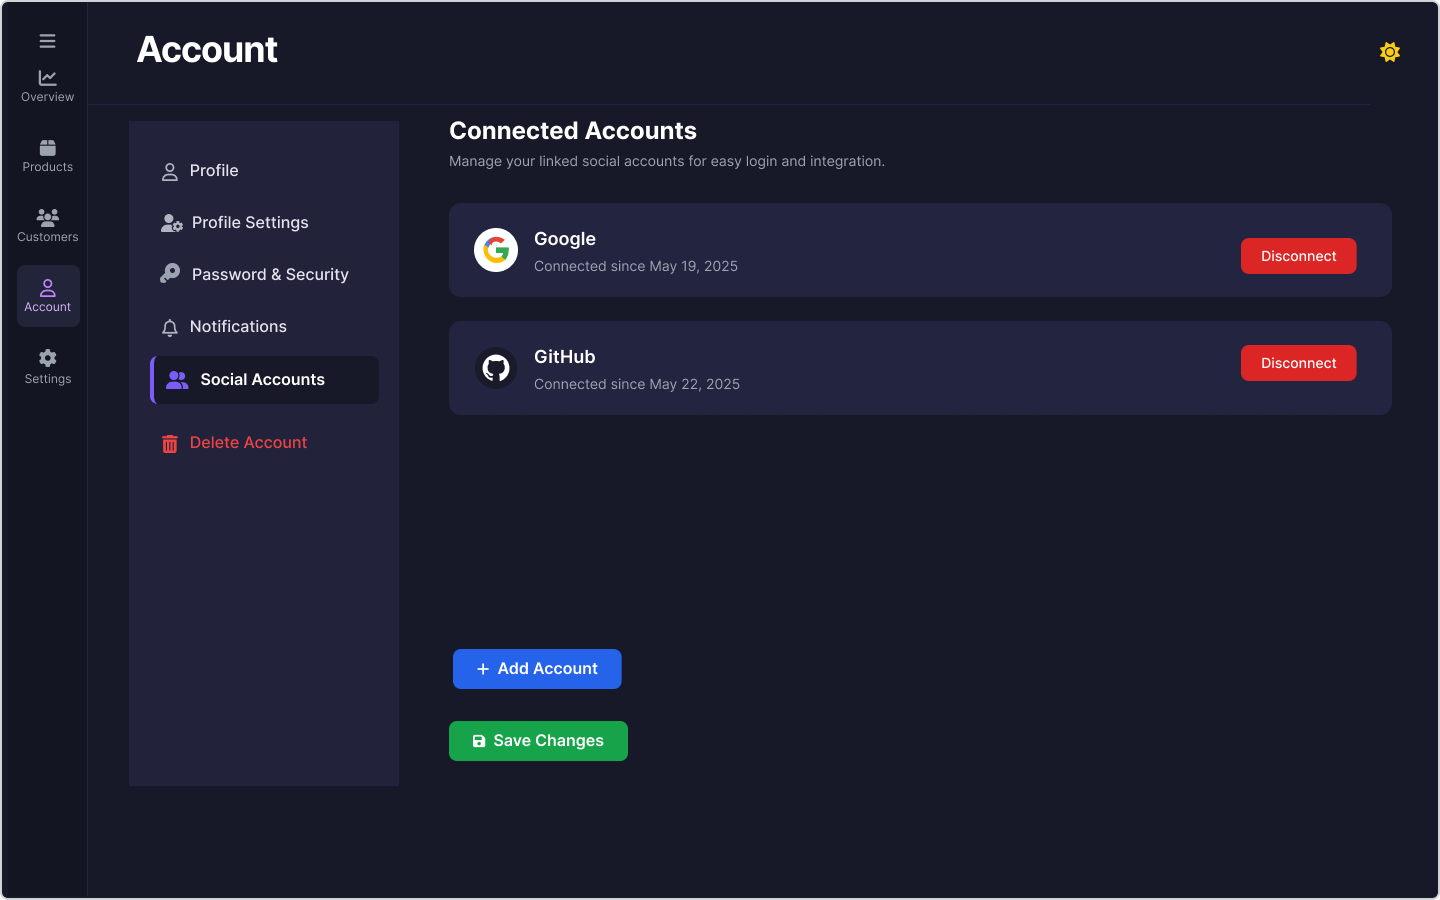
\includegraphics[width=0.8\textwidth]{pictures/admin/Connected_Accounts_Admin}
		\caption{Social Account page}\label{fig:figure8}
	\end{figure}
	This page provides the administrator with the ability to manage connections to various external social accounts such as Google, GitHub, and others. It displays a list of all currently connected accounts, including:
	\begin{itemize}
		\item \textbf{Account Provider} (e.g., Google, GitHub)
		\item \textbf{Date of Connection}
		\item \textbf{Status} (Connected/Disconnected)
	\end{itemize}
	Key Features:
	\begin{itemize}
		\item \textbf{Connect New Account:} A button or option allows the admin to link a new social account by authenticating with the selected provider.
		\textbf{Disconnect Account:} For each connected account, there is an option to disconnect or revoke access.
		\item \textbf{Connection History:} Displays the date and time when each account was connected.
	\end{itemize}
	The main purpose of this page is to give administrators full control over their linked external accounts, ensuring a secure and customizable login experience.
	
	
	\subsubsection{Delete Account}
	\begin{figure}[h]
		\centering
		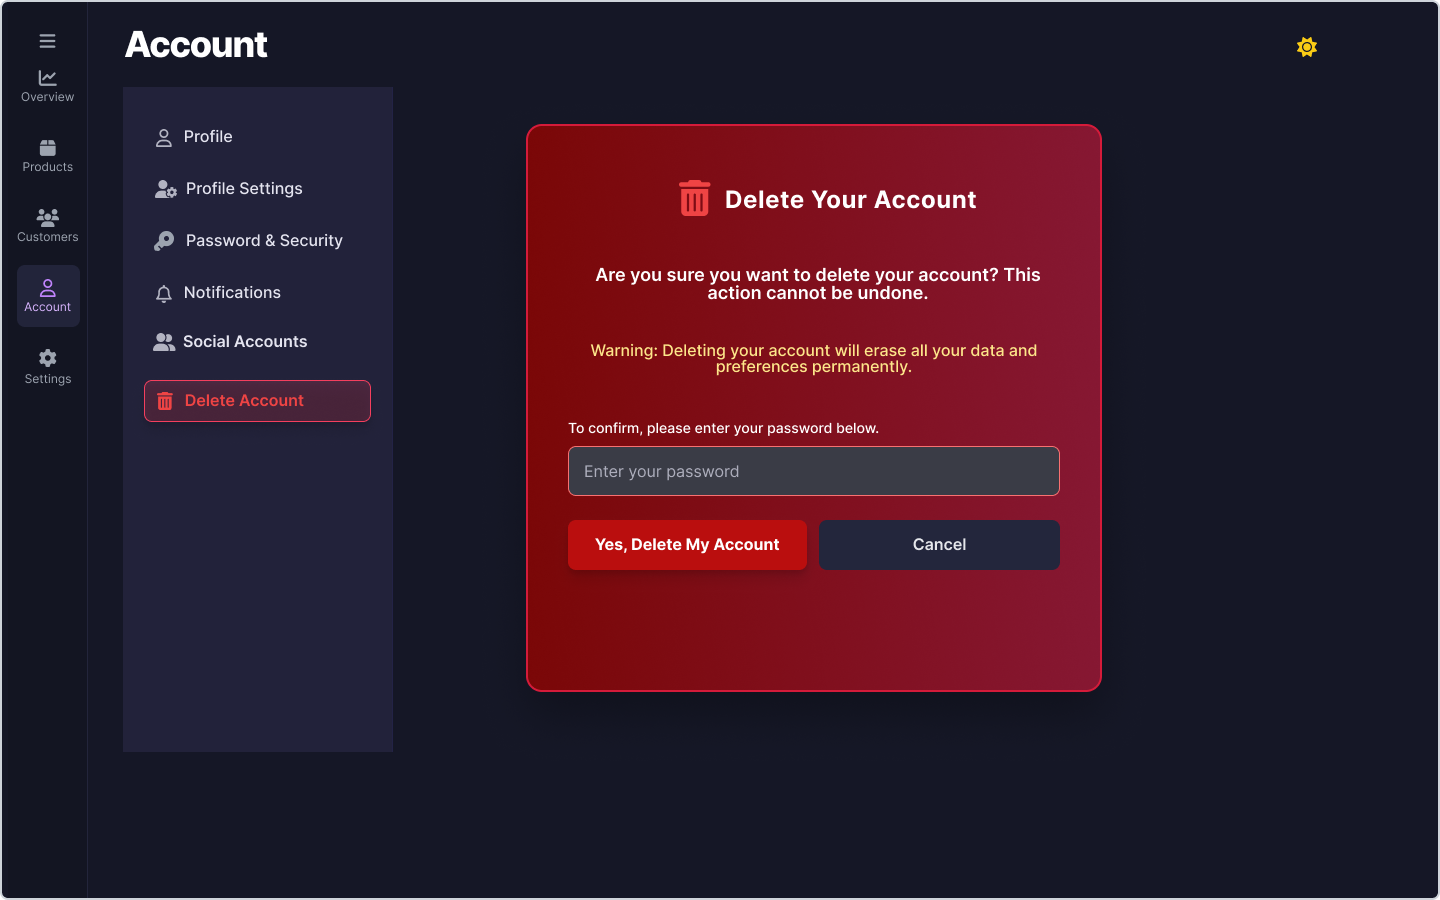
\includegraphics[width=0.8\textwidth]{pictures/admin/Delete_Admin}
		\caption{Delete Account page}\label{fig:figure9}
	\end{figure}
	This page allows the administrator to delete their personal account.
	To proceed, the administrator must enter their current password and then click the \textbf{"Yes, Delete My Account"} button or cancel the action.
	
	
	\subsection{Settings}\label{subsec:settings}
	
	\vspace{0.4cm}
	\begin{figure}[h]
		\centering
		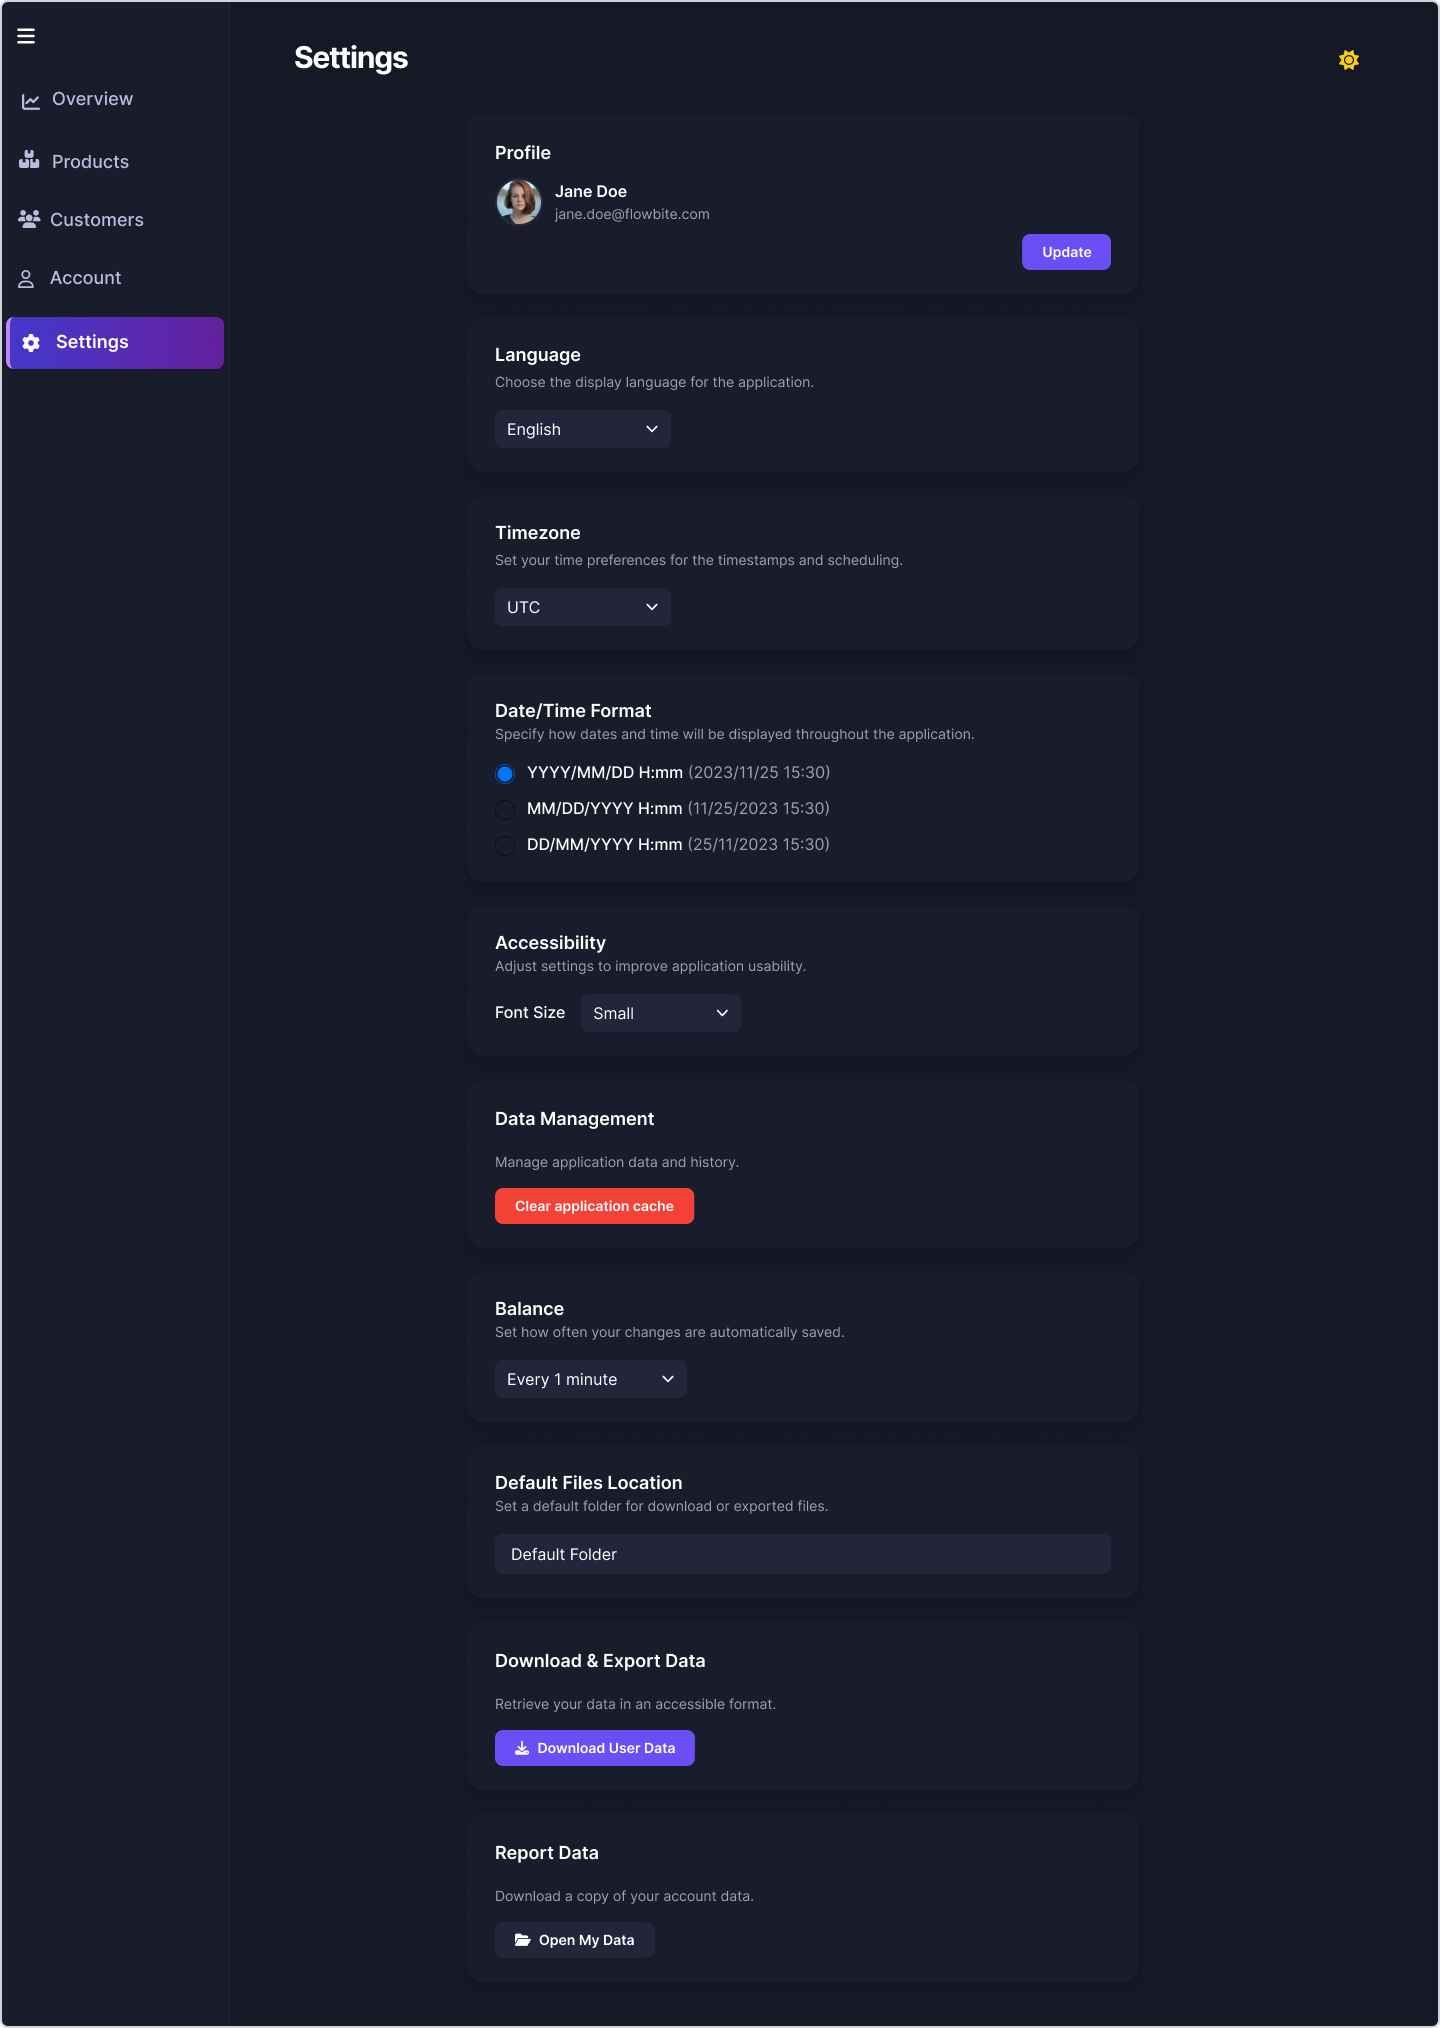
\includegraphics[width=0.6\textwidth]{pictures/admin/Settings_Admin}
		\caption{Settings page}\label{fig:figure10}
	\end{figure}
	
	This area consists of several distinct cards or sections, each focused on a specific category of settings:
	\begin{itemize}
		\item \textbf{Profile Section} - Contains a button labeled ``Update, '' which redirects the admin to the profile settings on the account page.
		\item \textbf{Language Section} - A dropdown menu for selecting the preferred language of the platform interface.
		\item \textbf{Timezone Section} - A dropdown menu for adjusting the system's timezone according to the admin’s location.
		\item \textbf{Date/Time Format Section} - Offers radio buttons to switch between different date/time display formats (e.g., DD/MM/YYYY or MM/DD/YYYY).
		\item \textbf{Accessibility Section} - A dropdown menu to change UI display size or enable accessibility features (e.g., larger text, high-contrast mode).
		\item \textbf{Data Management Section} - Provides an option to clear cache to free up storage and refresh data.
		\item \textbf{Balance Section} - A dropdown menu to set the auto-save frequency (e.g., every 5 minutes, 10 minutes).
		\item \textbf{Default Files Location Section:} Allows the admin to set the default folder for downloads or exported files.
		\item \textbf{Report Data Section:} Includes an ``Export Data'' button for downloading a complete copy of account-related data.
	\end{itemize}
	
	
	
	% ==========================================================
\section{Design Decisions \& Rationale}

In this section, we walk through the main design choices we made, explaining how each one supports the needs of our two primary users: \textbf{Regular Shoppers} and \textbf{Store Administrators}. Our goal was always to make the experience intuitive and efficient for everyone.

\subsection{Layout}
\begin{itemize}
	\item \textbf{Home Screen Flow}: We start with a clear welcome message, then introduce what we offer, and finally highlight a few featured categories in a carousel. This step‑by‑step approach helps new visitors discover and explore without feeling lost. (Regular Shoppers)
	\item \textbf{Flexible Product Grid}: No matter the screen size, our product cards keep the same proportions so items are easy to compare. Shoppers appreciate the consistency, and admins get a reliable preview of the catalog. (Regular Shoppers \& Administrators)
	\item \textbf{Two‑Column Detail Views}: For checkout and admin pages, we split the screen: one side shows details like your cart, and the other gives the summary. It’s easier on the eyes and speeds up decision‑making. (Regular Shoppers \& Administrators)
\end{itemize}

\subsection{Interaction Patterns}
\begin{itemize}
	\item \textbf{Always-Visible Top Bar}: Search, cart, and account buttons remain on screen at all times, allowing shoppers to switch effortlessly between browsing, their cart, and checkout with a single click. (Regular Shoppers)
	
	\item \textbf{Slide‑Out Filters}: On mobile, shoppers tap the hamburger icon; on desktop, a pill‑shaped button reveals filters. The page stays clean, and everyone can narrow down lists without losing context. (Regular Shoppers \& Administrators)
	\item \textbf{Quick‑Edit Modals}: In admin pages, small pop‑ups let you edit products or users right where you are, without loading a new page. It cuts down on clicks and keeps your workflow smooth. (Administrators)
\end{itemize}

\subsection{Colors}
\begin{itemize}
	\item \textbf{Bold Accent for Actions}: We chose a bright color for key buttons like “Shop Now” and “Save Changes.” It instantly grabs attention and guides users to the next step. (Regular Shoppers \& Administrators)
	\item \textbf{Calm, High‑Contrast Backgrounds}: Soft greys and clean whites let product images shine and ensure all text meets accessibility standards for contrast. (Accessibility)
	\item \textbf{Light and Dark Modes}: Whether you prefer a bright interface by day or a darker one at night, we’ve got you covered. It’s easier on the eyes and adapts to any environment. (Regular Shoppers \& Administrators)
\end{itemize}

\subsection{Typography}
\begin{itemize}
	\item \textbf{Simple Sans‑Serif Font}: We picked a modern font that’s easy to read at any size. Headings and body text use different weights so you can scan titles and details at a glance. (Regular Shoppers \& Administrators)
	\item \textbf{Readable Sizes and Spacing}: Body text is set to a comfy 16pt with generous line spacing. Larger headings help break up content and make busy pages feel more organized. (Accessibility)
\end{itemize}

\subsection{Accessibility}
\begin{itemize}
	\item \textbf{Keyboard Friendly}: You can navigate every button and link using just your keyboard. Visible focus outlines ensure you always know where you are. (Accessibility)
	\item \textbf{Screen‑Reader Support}: We added ARIA labels and roles to menus, dialogs, and forms so that assistive tech can read out exactly what’s happening. (Accessibility)
	\item \textbf{Respecting Reduced Motion}: Animations dial back automatically if you prefer minimal movement, reducing potential discomfort. (Accessibility)

\end{itemize}


	% ==========================================================
	\section{Responsiveness \& Accessibility}\label{sec:responsiveness-&-accessibility}
	Fluid CSS grid, break-points 1024 / 768 / 480 px, keyboard navigation, aria-labels, reduced-motion support.
	
	% ==========================================================
	\section{Acknowledgment of AI Technologies}\label{sec:acknowledgment-of-ai-technologies}
	Document drafted with GPT-4o assistance; final content reviewed and refined by the authors.
	
	% ==========================================================
	\section{Conclusion}\label{sec:conclusion}
	This portfolio meets all assignment requirements and provides a clear blueprint for development.
	






	
\end{document}